\documentclass{article}
\usepackage[a4paper, left=1.0in, right=1.0in, top=1.0in, bottom=1.0in]{geometry}
\usepackage{array}
\usepackage{bm}
\usepackage{amsmath}  % For advanced math typesetting
\usepackage{amsfonts} % For math fonts like \mathbb
\usepackage{amssymb}  % For symbols like \mathbb
\usepackage{tikz}     % For drawing matrices
\usetikzlibrary{trees}

\title{Introduction to Machine Learning Notes}
\author{Albert Jojo}
\date{\today}

\begin{document}

\maketitle

\section{Introduction}
This section will go over the basic machine learning algorithms.
Machine Learning (ML) is a subfield of AI, which focuses on studying the methods that can be used to improve the 
performance of a model over time.

\section{Classification Exercise}
\subsection{General Steps to Utilize and Train the Model}
\begin{enumerate}
    \item Load the dataset.
    \item Split the dataset into training and testing sets.
    \item Train the model.
    \item Evaluate the model performance.
\end{enumerate}
In this exercise, we are using the \textbf{Decision Tree Classifier} algorithm.

\subsection{How it Works}
The algorithm tries to find the best way to split the data at each step based on the features.
It looks for the splits that maximize the separation based on a feature. The best split is decided by
\textbf{Entropy}, which is a metric used for information gain. \textbf{Note:} A low entropy value indicates that the data
in that split is homogeneous, which is desired in a classification task.

\begin{center}
    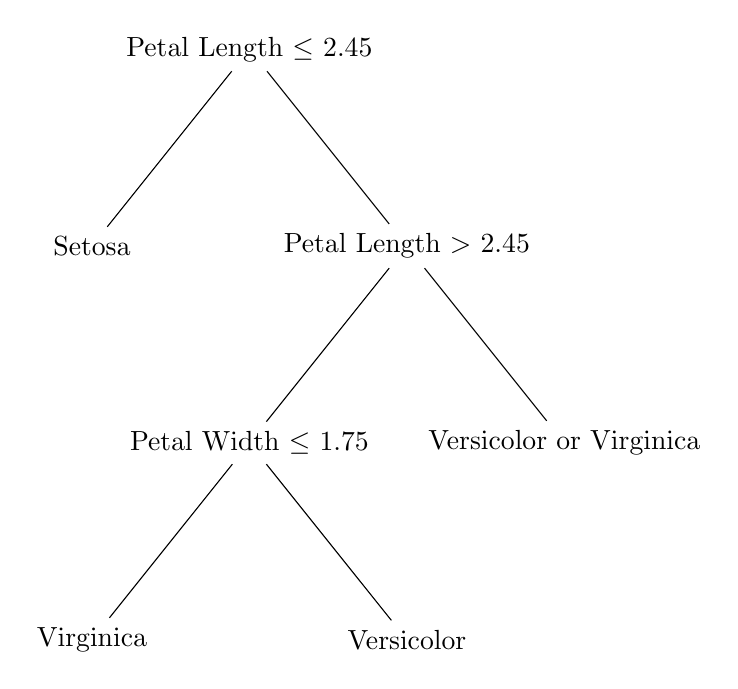
\begin{tikzpicture}[
        sibling distance=40mm,
        level distance=25mm
      ]
        \node {Petal Length $\leq$ 2.45}
          child { node {Setosa} }
          child { node {Petal Length $>$ 2.45}
            child { node {Petal Width $\leq$ 1.75}
              child { node {Virginica} }
              child { node {Versicolor} }
            }
            child { node {Versicolor or Virginica} }
          };
      \end{tikzpicture}  
\end{center}

\section{Definition of AI}
\begin{itemize}
  \item \textbf{Artificial Intelligence:} Intelligence exhibited by machines.
  \item \textbf{High-Profile Applications:}
  \begin{itemize}
    \item Advanced web search engines
    \item Recommendation systems
    \item Virtual assistants
    \item Autonomous driving
    \item Generative and creative tools
  \end{itemize}
  \item \textbf{Machine Learning:} A subset of AI that focuses on algorithms that allow computers to learn from data.
  \item \textbf{Deep Learning:} A subset of Machine Learning that utilizes artificial neural networks with multiple layers.
\end{itemize}

\section{ML with Big Data}
\begin{enumerate}
  \item \textbf{Observed Input-Output Mapping:} Observe some outputs $y_1, ... , y_T$ corresponding to input feature vectors $x_1, ..., x_T$.
  \item \textbf{Prediction:} A predictive model that takes in the input vectors and outputs a predictive value.
  \item \textbf{Supervised Learning:} Learning an input-output mapping based on labeled data.
  \item \textbf{Unsupervised Learning:} Learning patterns from data without labeled outputs.
  \item \textbf{Features:} The inputs.
  \item \textbf{Training:} The act of using data to find the best model.
  \item \textbf{Loss Function:} A function that assesses model quality, such as Mean Squared Error (MSE):
        \begin{equation}
        L = \frac{1}{T} \sum_{i=1}^{T} (y_i - \hat{y}_i)^2
        \end{equation}
        For classification, a common loss function is Cross-Entropy Loss:
        \begin{equation}
        L = -\sum_{i=1}^{T} \left[ y_i \log(\hat{y}_i) + (1 - y_i) \log(1 - \hat{y}_i) \right]
        \end{equation}
\end{enumerate}

\section{Two-Layer Neural Network}
A neural network aims to learn an underlying function from input data to output predictions. 
The basic formulation involves learning a function:
\[
y_i = f(x_i) + z_i
\]
where $z_i$ represents noise.

For example, fitting a polynomial of degree $k$:
\[
f(x, \theta) = \sum_{|\alpha| \leq k} \theta_{\alpha} x^{\alpha}
\]
where $\alpha$ represents a multi-index over feature dimensions.

To evaluate model quality, we define the expected risk:
\[
R(\theta) = \mathbb{E}\left[(f(x) - f(x,\theta))^2\right]
\]
and the empirical risk based on observed data:
\[
R_n(\theta) = \frac{1}{n}\sum_{i=1}^{n} (y_i - \hat{f}(x_i,\theta))^2.
\]

\subsection{Simple Neural Network Model}
A simple neural network approximates the function using multiple neurons:
\[
\hat{f}(x,\theta) = \frac{1}{N}\sum_{i=1}^{N} \sigma(x,\theta_i)
\]
where:
\begin{itemize}
  \item $N$ is the number of neurons (hidden units),
  \item $\sigma(x,\theta_i)$ is the activation function applied to each neuron,
  \item $\theta$ represents the network parameters.
\end{itemize}
Common activation functions include:
\begin{itemize}
  \item \textbf{Sigmoid:} $\sigma(x) = \frac{1}{1 + e^{-x}}$
  \item \textbf{ReLU:} $\sigma(x) = \max(0, x)$
\end{itemize}

\subsection{Stochastic Gradient Descent}
To minimize the empirical risk $R_n(\theta)$, we use Stochastic Gradient Descent (SGD):
\[
\theta \leftarrow \theta - \eta \nabla_{\theta} l(y_i, x_i, \theta)
\]
where $\eta$ is the learning rate and $l(y_i, x_i, \theta)$ is the loss function for a single data point. This iterative update gradually optimizes the model parameters.

\subsection*{Excess Risk}:
\[
L(\hat{\theta}) - \inf_{\theta \epsilon \theta}L(\theta) \leq  \frac{c}{n} + O(\frac{1}{n})
\]
where:
C: depends on the questions(constant)
O(1/n): rate of decreasing

\subsection*{Theorem}
\begin{itemize}
  \item 
  \[
    \sqrt{n}(\hat{\theta} - \theta_{real}) = O_p(1) \rightarrow \text{bounded in probability} \\
    P(\Vert \sqrt{n}(\hat{\theta} - \theta_{real})\Vert_2 > M) < \epsilon
  \]
  \item 
  \[
    \sqrt{n}(\hat{\theta} - \theta_{real}) \rightarrow^{d} N(0,)
  \]
  \item 
  \[
    \sqrt{n}(\hat{\theta} - \theta_{real}) = O_p(1) \rightarrow \text{bounded in probability} \\
    P(\Vert \sqrt{n}(\hat{\theta} - \theta_{real})\Vert_2 > M) < \epsilon
  \]
  
  
\end{itemize}

\section*{Parts of a Neural Network}
\begin{enumerate}
  \item Layers
  \item Activation Functions
  \item Loss Functions
  \item Neural Network
\end{enumerate}
\subsection*{Layers}
Layer: is a collection of neurons(nodes) that process data at a particular stage in the network. Consists of Input Layer, Hidden Layer, and Output Layer.
\subsubsection*{Abstract Layer}
This class serves as an abstract base class for all layers in the network.
\begin{itemize}
  \item **Forward Pass:** Computes the ouput of the layer given an input
  \item **Backward Pass:** Computes the gradients with respect to the input and parameters
  \item **Step:** Updates the layer parameters(weights and biases)
\end{itemize}
\subsubsection*{Linear Layers}
A layer of neural network, that performs a linear transformation on the input.
\[
y = x \cdot W + b
\]
\begin{itemize}
  \item \textbf{self.w}: Represents the weight matrix of shape (in\_dim, out\_dim), initialized using small random values.
  \item \textbf{self.b}: Bias vector of shape (1, out\_dim), initialized to zeros.
  \item \textbf{self.dw} \& \textbf{self.db}: Store the computed gradients of weights and biases during backpropagation.
\end{itemize}
\textbf{Forward Pass:}
\[
\textbf{out} = \textbf{inp} \cdot W + b
\]
\begin{itemize}
  \item \textbf{inp}: Input matrix of shape \((\texttt{batch\_size}, \texttt{in\_dim})\)
 \item \textbf{self.w}: Weight matrix \( \mathbf{W} \in \mathbb{R}^{\texttt{in\_dim} \times \texttt{out\_dim}} \)
  \item \textbf{self.b}: Bias **vector** of shape \((1, \texttt{out\_dim})\)  % Fixed terminology (vector, not matrix)
  \item \textbf{OUTPUT}: Matrix of shape \((\texttt{batch\_size}, \texttt{out\_dim})\)
\end{itemize}

\textbf{Backward Pass:}
\\ Computes the gradients needed for updating the weights and biases. Given the upstream gradient \(\text{up\_grad}\), we compute:

\begin{itemize}
  \item \textbf{Gradient w.r.t weights} (\(\frac{\partial L}{\partial W}\)):
  \[
  \frac{\partial L}{\partial W} = X^T \cdot \text{up\_grad}
  \]
  where:
  \begin{itemize}
    \item \( X \) represents the input from the previous layer.
    \item \( \text{up\_grad} \) is the gradient passed from the next layer.
    \item \( X^T \) (transpose of \( X \)) ensures proper matrix dimensions.
  \end{itemize}

  \item \textbf{Gradient w.r.t bias} (\(\frac{\partial L}{\partial b}\)):
  \[
  \frac{\partial L}{\partial b} = \sum \text{up\_grad}
  \]
  Since the bias does not depend on input values, its gradient is simply the sum of all elements in \(\text{up\_grad}\).

  \item \textbf{Gradient w.r.t input} (\(\frac{\partial L}{\partial X}\)) to be propagated to previous layers:
  \[
  \frac{\partial L}{\partial X} = \text{up\_grad} \cdot W^T
  \]
\end{itemize}

These gradients are used to update the model parameters using gradient descent:
\[
W = W - \eta \frac{\partial L}{\partial W}
\]
where \( \eta \) is the learning rate.
\vspace{.2cm}
\\ \textbf{Step Method}
Updates the weigths and biases using the computed gradients and learning rate(lr).
\[
W = W - lr \cdot \frac{\partial L}{\partial W}
\]
\[
b = b - lr \cdot \frac{\partial L}{\partial W}
\]
\subsection*{Activation Functions}
\subsubsection*{Sigmoid}
\[
f(x) = \frac{1}{1 + e^{-x}}
\]
\begin{itemize}
  \item This function squashes the input into the range [0,1] making it useful for binary classification tasks
  \item Converts any real-values number into probability like input
  \item It may cause vanishing gradients due to its flat slope for extreme values in deeper networks
\end{itemize}
\subsubsection*{ReLU(Rectified Linear Unit)}
\[
f(x) = max(0,x)
\]
\begin{itemize}
  \item Ouputs 0 if the input is less than zero, otherwise returns the input itself
  \item Helps introduce non-linearity into the model, essential for complex learning algorithms
  \item Helps avoid vanishing gradient problem, common in deep networks with Sigmoid activation
  \item During backpropagation only the gradients for inputs greater than 0 pass through:
  \[
  f'(x) = 
  \begin{cases}
    1 & \text{if } x > 0 \\
    0 & \text{otherwise}
  \end{cases}
  \]
\end{itemize}
\subsubsection*{Softmax}
\[
f(x_i) = \frac{e^{x_i}}{\sum_{j} e^{x_j}}
\]
\begin{itemize}
  \item Normalizes the input values into probabilities that sum to 1
  \item Used in the final layer of a neural network for multi-class classification
  \item Converts raw scores into probabilites where each class has a non-negative probability between 0 and 1
  \item Subtracting the maximum input value (np.max(inp)) from all inputs before applying np.exp helps prevent overflow errors.
\end{itemize}
\section*{Loss Functions}
\subsubsection*{Cross Entropy Loss}
\[
L = -\frac{1}{N}\sum_i\sum_{c}y_{ic}log(p_{ic})
\]
Typically used in classification tasks since it measures the dissimilarity between the true distrbution(target) and
the predicted probability distribution(prediction).
\subsubsection*{Mean Squared Error(MSE)}
\[
L = \frac{1}{N}\sum_i(p_i - y_i)^2
\]
Is primarily used for regression tasks, where you need to measure the distance between the predicted, continuous values and true values.
\end{document}
